	\documentclass[10pt,oneside]{CBFT_book}
	% Algunos paquetes
	\usepackage{amssymb}
	\usepackage{amsmath}
	\usepackage{graphicx}
	\usepackage{libertine}
	\usepackage[bold-style=TeX]{unicode-math}
	\usepackage{lipsum}

	\usepackage{natbib}
	\setcitestyle{square}

	\usepackage{polyglossia}
	\setdefaultlanguage{spanish}


	\usepackage{CBFT.estilo} % Cargo la hoja de estilo

	% Tipografías
	% \setromanfont[Mapping=tex-text]{Linux Libertine O}
	% \setsansfont[Mapping=tex-text]{DejaVu Sans}
	% \setmonofont[Mapping=tex-text]{DejaVu Sans Mono}

	%===================================================================
	%	DOCUMENTO PROPIAMENTE DICHO
	%===================================================================

\begin{document}

% =================================================================================================
\chapter{Método de separación de variables}
% =================================================================================================

% =================================================================================================
\section{Separación de variables}
% =================================================================================================

Separamos los problemas en regiones donde vale $\lapm{\phi} = 0$ entonces las fronteras tendrán la
$\rho(\vb{x}')$ en general en forma de $\sigma,\lambda$.

Para coordenadas cartesianas intentaremos resolver $\lapm{\phi} = 0$, es decir
\[
	\dpar[2]{\phi}{x} + \dpar[2]{\phi}{y}  + \dpar[2]{\phi}{z}  = 0
\]
pidiendo
\[
	\phi(x,y,z) = X(x)Y(y)Z(z)
\]
de manera que 
\[
	\frac{1}{X}\dtot[2]{X}{x} + \frac{1}{Y}\dtot[2]{Y}{y} + \frac{1}{Z}\dtot[2]{Z}{z} = 0 \qquad 
	- \alpha^2  - \beta^2 + \gamma^2 = 0 \quad \Rightarrow  \gamma^2 = \alpha^2 + \beta^2 
\]
cada término es una constante. La solución general es
\[
	\phi(x,y,z) = \sum_{m=0}^\infty \sum_{n=0}^\infty A_{m,n} \euler^{\pm i\alpha_m x}
	\euler^{\pm i\beta_n y} \euler^{\pm i\sqrt{\alpha_m^2 + \beta_n^2 }z}
\]
donde habrá que adaptar según las condiciones de contorno. Se da que $A_{m,n}$ es una constante general
y hay condiciones periódicas en $x,y$
\[
	A\euler^{\pm i\alpha x} = A_\alpha \cos(\alpha x) + B_\alpha \sin(\alpha x)
\]
corresponde a condiciones de potencial periódicas, cuando necesito dos ceros por ejemplo (ver ilustración
lateral --que falta--)
\[
	A\euler^{\pm \gamma z} = A_\gamma \cosh(\gamma z) + B_\gamma \sinh(\gamma z)
\]
corresponde a atravesar densidades de carga.

Para coordenadas esféricas es
\[
	\frac{1}{r} \frac{\partial}{\partial r}\left( r^2 \dpar{\phi}{r} \right) + 
	\frac{1}{r^2 \sin(\theta)}\frac{\partial}{\partial\theta}\left(\sin(\theta)\dpar{\phi}{\theta}\right)+
	\frac{1}{r^2 \sin(\theta)} \dpar[2]{\phi}{\varphi} = 0
\]
proponiéndose la separación
\[
	\phi(r,\theta,\varphi) = R(r) \Theta(\theta) Q(\varphi)
\]
siendo
\[
	Y(\theta,\varphi) = \Theta(\theta) Q(\varphi)
\]
un armónico esférico.
Tenemos un oscilador armónico en $\varphi$,
\[
	Q = \euler^{\pm i\alpha \varphi}
\]
si usamos $0\leq \varphi \leq 2\pi$ de modo que $\alpha\in\mathbb{Z}$ y entonces $\alpha=m$, con simetría
azimutal es $m=0$ (rotación en $\varphi$), 
\[
	Q = G\varphi + H \qquad\qquad  G,H \quad ctes.
\]
Para las otras funciones será
\[
	R(r) = A_\ell r^\ell + B_\ell R^{-\ell-1}
\]
\[
	\Theta(\theta) = C_\ell P_\ell^m (\cos(\theta)) + D_\ell Q_\ell^m (\cos(\theta))
\]
siendo $P_\ell^m$ polinomio de Legendre, que verifica la fórmula de Rodrigues
\[
	P_\ell (x) = \frac{1}{2^\ell \ell!} \frac{d^\ell}{d x^\ell} [x^2 - 1]^\ell
\]
con $P_\ell(\cos(\theta))$ polinomio de Legendre de primera especie, y $Q_\ell(\cos(\theta))$ de segunda
especie.
Los $\{ P_\ell\}$ son un conjunto completo y ortogonal en $-1 \leq x \leq 1$ o bien en $0\leq \theta\leq \pi$.

Los $\{ Q_\ell^m(\cos(\theta))\}$ tienen problemas en $\theta=0,\theta=\pi$ (eje $z$) de manera que si está el
eje $z$ no podemos usar $Q_\ell^m$; en estos problemas sólo podemos usar $P_\ell^m(\cos(\theta))$.
\[
	\phi(r,\theta,\phi) = \sum_{\ell=0}^{\infty}\sum_{m=-\infty}^{\infty} \left[ A_\ell r^\ell + 
	B_\ell r^{-\ell-1} \right] \left[ C_\ell P_\ell^m + D_\ell Q_\ell^m \right] \left[ E_m \cos(m\phi) + 
	F_m \sin(m\phi) \right]
\]
y en el caso particular $m=0$
\[
	\phi(r,\theta,\phi) = \sum_{\ell=0}^{\infty}\sum_{m=-\infty}^{\infty} \left[ A_\ell r^\ell + 
	B_\ell r^{-\ell-1} \right] \left[ C_\ell P_\ell^m + D_\ell Q_\ell^m \right] \left[ G_0 \phi + 
	H_0 \right]	
\]
Las constantes $A_\ell, B_\ell, C_\ell, D_\ell, E_m, F_m$ se ajustan con el $\phi (r\to\infty)$, 
$\phi (r\to 0)$, $\phi (z = 1)$ y $\phi (z = -1)$.

Lo que permite esquivar el problema del punto singular en $x \equiv \cos(\theta)=1$ es
\[
	\beta^2 = \ell(\ell + 1) \qquad - \ell < m < \ell \qquad \alpha^2 = m^2
\]

Recordemos las sumas de series
\[
	\frac{1}{1-z} = \sum_{\ell=0}^{\infty} z^\ell \qquad \frac{1}{1+z} = \sum_{\ell=0}^{\infty} (-1)^\ell 
	z^\ell	\qquad |z|<1,
\]
el polinomio asociado de Legendre
\[
	P_\ell^m (x) =) \frac{(-1)^m}{2^\ell \ell!} [1-x^2]^{m/2} \frac{d^{\ell + m}}{dx^{\ell + m}} 
			[x^2 -1]^\ell
\]
que cumple
\[
	P_\ell (1) = 1 \quad P_\ell (-1) = (-1)^\ell \qquad  \forall \ell
\]
con 
\[
	\int_{-1}^1 [P_\ell (x)]^2 \: dx = \frac{2}{ 2\ell + 1 }
\]
siendo la ortogonalidad
\[
	\int_0^\pi P_{\ell'}^m (\cos(\theta)) P_\ell^m (\cos(\theta)) \sin(\theta) \: d\theta = 
	\delta_{\ell\ell'}
\]
\[
	\int_{-1}^{+1} P_{\ell'}^m (x) P_\ell^m (x) \: dx= \frac{2}{2\ell + 1}
	\frac{(\ell + m)!}{(\ell - m)!} \: \delta_{\ell\ell'}
\]

En esféricas las constantes de separación están asociadas
\[
	R(r) \; \mathrm{con} \; \ell \qquad \Theta(\theta) \; \mathrm{con} \; \ell,m \qquad
	Q(\phi) \; \mathrm{con} \; m
\]

% =================================================================================================
\section{Detalles sobre solución de problemas de potencial}
% =================================================================================================

Si el potencial es par en una coordenada, entonces uso funciones pares (cosenos). 
La continuidad del potencial
\[
	\phi_I(x=0) = \phi_{II}(x=0) = 
\]
y salto en el campo
\[
	\left.\dpar{\phi_I}{x} - \dpar{\phi_{II}}{x}\right|_{x=0} = -4\pi\sigma|_{x=0}
\]

\begin{figure}[htb]
	\begin{center}
	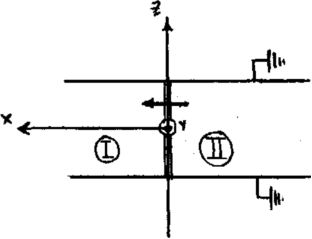
\includegraphics[width=0.4\textwidth]{images/fig_ft1_potencial.pdf}	 
	\end{center}
	\caption{}
\end{figure} 
Si tengo condiciones periódicas en la coordenada irán senos y cosenos trigonométricos, entonces se
discretizan $m,n$ y tengo $\sum_n \sum_m$ una serie de Fourier.

Si tengo condiciones no periódicas en la coordenada irán seno, coseno hiperbólicos entonces tengo
$\int dk$ integral de Fourier.

En general tomo
\[
	\alpha^2 + \beta^2 = \gamma^2
\]
pudiéndose discretizar los $k's$ luego. Se considera $\alpha^2 \equiv k_{\hat{e}_1}^2$ y así siguiendo
con las otras dos.

Sobre la ecuación de salto en el campo aplicamos ortogonalidad y despejamos coeficientes en función
de $\sigma$.

Detalle: el salto en el campo se hace siguiendo la normal, como se ilustra abajo
\begin{figure}[htb]
	\begin{center}
	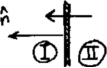
\includegraphics[width=0.3\textwidth]{images/fig_ft1_potencialsketch.pdf}
	\end{center}
	\caption{}
\end{figure} 
\[
	E_I^{\hat{n}} - E_{II}^{\hat{n}} = 4 \pi \sigma \qquad\qquad 
	- \dpar{\phi_I}{x} + \dpar{\phi_{II}}{x} = 4 \pi \sigma
\]

Para $k_{\hat{e}_1}^2$ en el caso discreto
\[
	\sum_{m=0}^\infty \cos(k_m e_1) + \sin(k_m e_1)
\]
pero en el continuo 
\[
	\int_{\infty}^{\infty} \euler^{ike_1} dk
\]
usamos $exp(ike_1)$ para que la integral converja en lugar de $(\cos(ke_1) + \sin(ke_1))$.

% =================================================================================================
\section{Expansiones ortonormales}
% =================================================================================================

\[
	\int_a^b U^*_n U_m d\xi = \delta_{mn} \qquad U_i \; mathrm{ortonormales}
\]
entonces en $(a,b)$ se da que la serie 
\[
	f(\xi) = \sum_{n=0}^\infty a_n U_n(\xi) 
\]
converge, donde  
\[
	a_n = \int_a^b U^*_n f(\xi) d\xi.
\]
La clausura es
\[
	\sum_{n=1}^\infty U^*_n(\vb{x}') U_n(\vb{x}) = \delta(\vb{x}-\vb{x}')
\]

\begin{figure}[thb]
	\begin{center}
	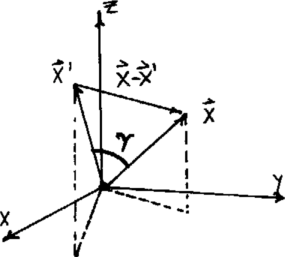
\includegraphics[width=0.4\textwidth]{images/fig_ft1_expansiones1.pdf}	 
	\end{center}
	\caption{}
\end{figure} 

Es útil el desarrollo
\[
	\frac{1}{|\vb{r} - \vb{r}'|} = \frac{1}{\sqrt{r^2 + r'^2 -2rr'\cos(\gamma)}}
	= \sum_{\ell=0}^\infty \frac{r^\ell_{<}}{r^\ell_{>}} P_\ell (\cos(\gamma))
\]
en polinomios de Legendre para el ángulo entre vectores en coordenadas esféricas.
En coordenadas esféricas, donde $\gamma=\gamma(\theta,\phi)$ es el ángulo entre vectores,
que surge del teorema del coseno.

\subsection{Prolongación analítica}

Consiste en {\it prolongar} una solución restringida por ejemplo en el eje polar a todo el
resto del espacio pegándole los polinomios de Legendre.
Lo ponemos en serie (pasamos un cálculo de F3 a una serie)
\[
	\phi(r,\phi/2) = \frac{Q}{\sqrt{r^2 + a^2}} = \sum_{\ell=0}^\infty Q \frac{a^\ell}{r^{\ell + 1}} 
	P_\ell (0) \qquad r > a
\]
\[
	\phi(r,\phi/2) = \frac{Q}{\sqrt{r^2 + a^2}} = \sum_{\ell=0}^\infty Q \frac{r^\ell}{a^{\ell + 1}} 
	P_\ell (0) \qquad r < a
\]
y $P_\ell(0)$ tiene términos pares solamente (los impares son nulos).

\begin{figure}[htb]
	\begin{center}
	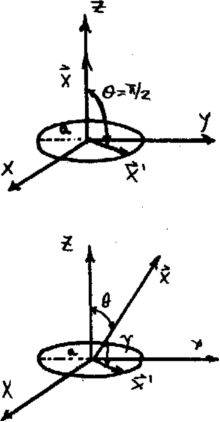
\includegraphics[width=0.3\textwidth]{images/fig_ft1_expansiones2.pdf}	 
	\end{center}
	\caption{}
\end{figure} 

Entonces
\[
	\phi(r,\phi/2) = \frac{Q}{a} \sum_{n=0}^\infty \frac{r^{2n}}{a^{2n}} P_{2n} (0) 
\]
con 
\[
	P_{2n} (0) = (-1)^n \frac{(2n-1)!}{2^n n!}
\]
por lo tanto para todo el espacio será

\begin{figure}[htb]
	\begin{center}
	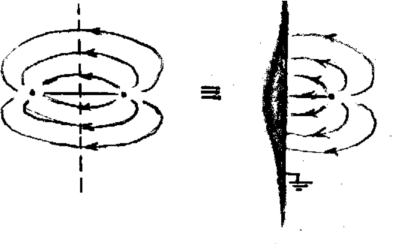
\includegraphics[width=0.4\textwidth]{images/fig_ft1_expansiones3.pdf}	 
	\end{center}
	\caption{}
\end{figure} 

\[
	\phi(r,\phi/2) = \frac{Q}{a} \sum_{n=0}^\infty \left( \frac{r}{a}\right)^{2n} P_{2n} (0) P_{2n} 
	(\sin(\theta)) \qquad r < a
\]
El hecho de que sólo vivan $\ell$ pares viene porque $\phi$ es par pues hay simetría de reflexión en el
plano $xy$, lo que sucede de $(0,\pi/2)$ es igual a lo que sucede de $(\pi/2, \pi)$.

Los problemas con simetría de revolución en torno a $\hat{z}$ pueden ser resueltos con el método de
prolongación analítica. La idea central es que si dos soluciones del potencial coinciden en un conjunto
de puntos (como ser el eje azimutal) entonces deben ser la misma solución.

\subsection{Comentario multipolos}

Estos dos problemas son equivalentes, pero multipolarmente tienen desarrollos diferentes.
El problema es que el metal a tierra tendrá carga hasta el infinito y entonces no podemos tener un
radio de convergencia.


% =================================================================================================
\section{Armónicos esféricos}
% =================================================================================================

\[
	Y_{\ell,m}(\theta,\varphi) = \sqrt{ \frac{ 2\ell + 1}{4\pi} \frac{(\ell-m)! }{(\ell+ m)! } }
	P_\ell^m(\cos(\theta)) \euler^{i m \varphi}
\]
Los armónicos esféricos son un conjunto ortonormalizado en 
\[
	- 1 \leq \cos(\theta) \leq 1 , \qquad 0 \leq \varphi \leq 2\pi
\]
\[
	Y_{\ell,-m}(\theta,\varphi) = (-1) Y_{\ell,m}^*(\theta,\varphi)
\]

La ortonormalidad
\[
	\int_0^{2\pi} d\varphi \int_0^\pi \sin(\theta) Y_{\ell,m}(\theta,\varphi) Y_{\ell,m}^*(\theta,\varphi) d\theta 
	= \delta_{\ell'\ell}\delta_{m'm}
\]
La completitud
\[
	\sum_{\ell=0}^\infty \sum_{m=-\ell}^\ell Y_{\ell,m}(\theta,\varphi) Y_{\ell,m}^*(\theta,\varphi) = 
\delta(\varphi 	-\varphi') \delta(\cos(\theta)-\cos(\theta'))
\]
Entonces una función $f$ cualquiera $\in L^2$ se puede expresar en armónicos esféricos,
\[
	f(\theta,\varphi) = \sum_{\ell=0}^\infty \sum_{m=-\ell}^\ell A_{\ell,m} Y_{\ell,m}(\theta,\varphi)
\]
de manera que el potencial en coordenadas esféricas es
\[
	\phi(r,\theta,\varphi) = \sum_{\ell=0}^\infty \sum_{m=-\ell}^\ell [A_{\ell,m}r^\ell + B_{\ell,m} r^{-(\ell+1)}] 
	Y_{\ell,m}(\theta,\varphi)
\]

Con respecto a la Figura, 

\begin{figure}[bht]
	\begin{center}
	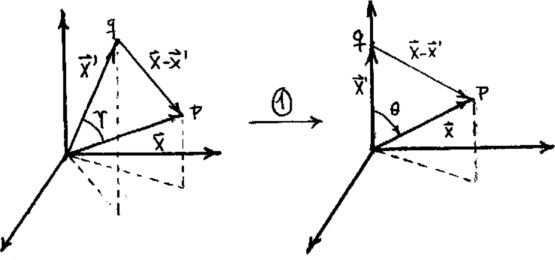
\includegraphics[width=0.7\textwidth]{images/fig_ft1_armesf1.pdf}	 
	\end{center}
	\caption{}
\end{figure} 

si $q$ está en $\hat{z}$ entonces simetría de revolución ($\gamma \to \theta$). Si por el contrario ,
$\gamma $ es nulo entonces simetría de revolución.

\begin{figure}[tb]
	\begin{center}
	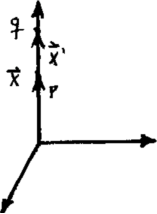
\includegraphics[width=0.3\textwidth]{images/fig_ft1_armesf2.pdf}	 
	\end{center}
	\caption{}
\end{figure} 

Un poco de álgebra de coordenadas,
\[
	\frac{1}{|\vb{x}-\vb{x}'|} = \frac{1}{\sqrt{r^2 + {r'}^2  - 2rr'\cos(\gamma)}} \Rightarrow
	\frac{1}{\sqrt{r^2 + {r'}^2  - 2rr'\cos(\theta)}}
\]
donde $|\vb{x}|=r$ y $|\vb{x}'|=r'$. Así
\[
	\left. \frac{1}{|\vb{x}-\vb{x}'|} \right|_{\gamma=0} = \frac{1}{\sqrt{r^2 + r'^2 -2rr'}}=
	\frac{1}{|r-r'|}
\]
luego si $r'<r$ será
\[
	\frac{1}{|r-r'|} = \frac{1}{r(1 - r'/r )} = \frac{1}{r} \sum_{\ell=0}^\infty \left(\frac{r'}{r}\right)^\ell = 
	\sum_{\ell=0}^\infty \frac{r'^\ell}{r^{\ell+1}}
\]
en cambio si es $r'>r$
\[
	\frac{1}{|r-r'|} = \frac{1}{r'(1 - r/r' )} = \frac{1}{r'} \sum_{\ell=0}^\infty \left(\frac{r}{r'}\right)^\ell = 
	\sum_{\ell=0}^\infty \frac{r^\ell}{r'^{\ell+1}}
\]
de manera que
\[
	\left. \frac{1}{|\vb{x}-\vb{x}'|} \right|_{\gamma=0} = \sum_{\ell=0}^\infty  \frac{r_<^\ell}{r_>^{\ell+1}}
\]
y podemos pensar en $1=P_\ell(1) \forall \ell$ y $1=P_\ell(\cos 0)$
\[
	\left. \frac{1}{|\vb{x}-\vb{x}'|} \right|_{\gamma=0} = \sum_{\ell=0}^\infty  \frac{r_<^\ell}{r_>^{\ell+1}}
	P_\ell(\cos 0)
\]
que será el $\phi$ de una carga unitaria en $\hat{z}$ y evaluado en $\hat{z}$.
Hacemos de esta manera prolongación analítica,
\[
	\frac{1}{|\vb{x}-\vb{x}'|}  = \sum_{\ell=0}^\infty  \frac{r_<^\ell}{r_>^{\ell+1}}
	P_\ell(\cos \gamma)
\]
y decimos que será el $\phi$ de una carga unitaria en cualquier parte (descompuesto en polinomios de Legendre).
Aquí $\gamma=\gamma(\theta,\varphi)$ y se puede llegar a una descomposición similar utilizando armónicos esféricos.

El potencial $\phi$ descompuesto en armónicos esféricos es
\[
	\frac{1}{|\vb{x}-\vb{x}'|}  = \sum_{\ell=0}^\infty \sum_{m=-\ell}^\ell \frac{r_<^\ell}{r_>^{\ell+1}}
	\frac{4\pi}{2\ell+1} Y_{\ell,m}(\theta,\varphi) Y_{\ell,m}^*(\theta',\varphi')
\]
y el teorema de adición de los armónicos esféricos ha sido usado
\[
	P_\ell(\cos \gamma) = \sum_{m=-\ell}^\ell \frac{4\pi}{2\ell+1} Y_{\ell,m}(\theta,\varphi) 
	Y_{\ell,m}^*(\theta',\varphi')
\]

\[
	\phi(\vb{x})= \int_{V'} \rho(\vb{x}')\left[ \sum_{\ell=0}^\infty \sum_{m=-\ell}^\ell 
	\frac{r_<^\ell}{r_>^{\ell+1}}\frac{4\pi}{2\ell+1} Y_{\ell,m}(\theta,\varphi) 
	Y_{\ell,m}^*(\theta',\varphi')\right] dV',
\]
que se puede cosmetizar como
\[
	\phi(\vb{x})= 4\pi \sum_{\ell=0}^\infty \sum_{m=-\ell}^\ell \frac{1}{2\ell+1} \left[
	\int_{V'} \rho(\vb{x}') Y_{\ell,m}^*(\theta',\varphi') {r'}_<^\ell dV' \right] 
	\frac{Y_{\ell,m}(\theta,\varphi) }{r_>^{\ell+1}},
\]
definiéndose el corchete como $q_{\ell m}$ coeficiente multipolar de orden $\ell m$, así
\[
	\phi(\vb{x})= 4\pi \sum_{\ell=0}^\infty \sum_{m=-\ell}^\ell \frac{q_{\ell m}}{2\ell+1} 
	\frac{Y_{\ell,m}(\theta,\varphi) }{r_>^{\ell+1}}.
\]

Entonces
\[
	\phi_{\ell m}(\vb{x})= 4\pi \frac{q_{\ell m}}{2\ell+1}\frac{Y_{\ell,m}(\theta,\varphi) }{r_>^{\ell+1}}
\]
y consecuentemente
\[
	\vb{E}_{\ell m}(\vb{x}) = - \Nabla \phi_{\ell m}(\vb{x})
\]

% =================================================================================================
\section{Separación de variables en cilíndricas}
% =================================================================================================

Se propone
\[
	\phi(\rho,\phi,z) = R(\rho) Q(\phi) Z(z)
\]
de modo que
\[
	\frac{1}{R} \dtot[2]{R}{\rho} + \frac{1}{R\rho} \dtot{R}{\rho} + \frac{1}{Q\rho^2} \dtot[2]{Q}{\phi} 
				+ \frac{1}{Z} \dtot[2]{Z}{z} = 0
\]
donde los primeros dos términos conducen a la ecuación de Bessel, el tercero es igual a $-\nu^2$ y el
cuarto a $k^2$. Sacamos
\[
	Z = \euler^{\pm kz}
\]
\[
	Q = \euler^{\pm i \nu \phi}
\]
donde si $0\leq \phi \leq 2\pi$ entonces $\nu \in \mathbb{Z}$. Si en cambio la variable $\phi$ no corre 
entre $0$ a $2\pi$ se dará que $\nu \notin \mathbb{Z}$.

\begin{center}
	\begin{tabular}{|c|c|}
	\hline
	$ \nu \in \mathbb{Z} $ & $ \nu \notin \mathbb{Z}  $ \\
	\hline
	$J_\nu(k\rho)$ & $J_\nu(k\rho)$ \\
	$J_{-\nu}(k\rho)$ & $N_\nu(k\rho)$ \\
	\hline
	\end{tabular} 
\end{center}




% \bibliographystyle{CBFT-apa-good}	% (uses file "apa-good.bst")
% \bibliography{CBFT.Referencias} % La base de datos bibliográfica

\end{document}
